\subsection{Radio frequency}

The RF section consists of a pair of RF coils, a 50~$\Omega$ current-sense resistor,
and an RF power amplifier. The RF coils are mounted on the outside of the cell heater,
with their axis perpendicular to the static magnetic field $B_0$.
 
\begin{figure}[h]
    \centering
    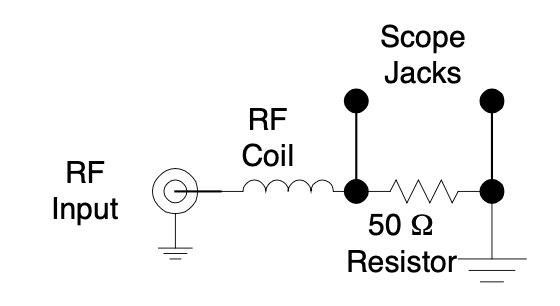
\includegraphics[width=0.5\textwidth]{figures/RF.png}
    \caption{RF coil pair and 50~$\Omega$ current-sensing resistor circuit.}
\end{figure}
 
\subsubsection*{RF Coil Specifications}
 
The RF coil pair is not in a Helmholtz configuration. Their properties are:
 
\begin{table}[h]
    \centering
    \begin{tabular}{lc}
        \hline
        Parameter & Value \\
        \hline
        Turns per side      & 3 \\
        Wire gauge          & 18~AWG copper \\
        Coil diameter       & 6.45~cm \\
        Coil separation     & 10.80~cm \\
        Inductance $L$      & 1.66~$\mu$H \\
        Parallel capacitance $C$ & 24~pF \\
        \hline
    \end{tabular}
    \caption{RF coil specifications.}
\end{table}
 
\subsubsection*{Coil Impedance and Self-Resonance}
 
The impedance of the RF coil as a function of angular frequency $\omega$ is:
\begin{equation}
    Z_{\text{coil}}(\omega) = j\omega L + \frac{1}{j\omega C}
    = j\left(\omega L - \frac{1}{\omega C}\right)
\end{equation}
The coil self-resonates when $Z_{\text{coil}} = 0$, i.e.:
\begin{equation}
    \omega_0 = \frac{1}{\sqrt{LC}}
\end{equation}
Substituting $L = 1.66\ \mu$H and $C = 24$~pF:
\begin{equation}
    f_0 = \frac{\omega_0}{2\pi} = \frac{1}{2\pi\sqrt{LC}}
        = \frac{1}{2\pi\sqrt{1.66\times10^{-6}\times24\times10^{-12}}}
        \approx 25\ \text{MHz}
\end{equation}
Below $f_0$, the coil behaves as a pure inductance; above $f_0$, the parallel
capacitance dominates. The operating frequency range of the amplifier is
10~kHz -- 30~MHz, well below the self-resonance frequency.
 
\subsubsection*{RF Magnetic Field Amplitude}
 
The RF current $I_{\text{rf}}$ flowing through the coils produces a transverse
oscillating magnetic field at the cell. For a single-turn coil of radius $r$ at the
centre, the field amplitude is:
\begin{equation}
    B_{\text{rf}} = \frac{\mu_0 N I_{\text{rf}}}{2r}
\end{equation}
where $N = 3$ is the number of turns per side. The RF current is measured from the
voltage $V_{50}$ across the 50~$\Omega$ sense resistor in series with the coil:
\begin{equation}
    I_{\text{rf}} = \frac{V_{50}}{50\ \Omega}
\end{equation}
so the RF field amplitude is:
\begin{equation}
    B_{\text{rf}} = \frac{\mu_0 N}{2r} \cdot \frac{V_{50}}{50}
\end{equation}
Note that at high frequencies the long cable and finite coil impedance cause the voltage
at the amplifier output to differ significantly from $V_{50}$; the sense resistor
measurement must therefore always be used for quantitative determination of
$B_{\text{rf}}$.
 
\subsubsection*{Rabi Frequency and Transition Probability}
 
The transverse RF field drives magnetic dipole transitions with $\Delta M = \pm 1$.
In the rotating-wave approximation, the on-resonance Rabi frequency is:
\begin{equation}
    \Omega_R = \gamma \frac{B_{\text{rf}}}{2}
             = \frac{g_F\,\mu_0}{\hbar}\cdot\frac{B_{\text{rf}}}{2}
\end{equation}
The transition probability between adjacent Zeeman sublevels after an interaction time
$t$ is:
\begin{equation}
    P_{M \to M\pm1}(t) = \sin^2\!\left(\Omega_R t\right)
\end{equation}
At resonance, a $\pi$-pulse of duration $t_\pi = \pi/\Omega_R$ inverts the population
completely. The optimum RF amplitude for maximum transition probability satisfies:
\begin{equation}
    \Omega_R \cdot \tau_{\text{transit}} = \frac{\pi}{2}
    \quad\Longrightarrow\quad
    B_{\text{rf}}^{\text{opt}} = \frac{\pi\,\hbar}{g_F\,\mu_0\,\tau_{\text{transit}}}
\end{equation}
where $\tau_{\text{transit}}$ is the effective interaction time of the atoms with the
RF field.
 
\subsubsection*{Off-Resonance Lineshape}
 
At a detuning $\Delta\omega = \omega - \omega_0$ from resonance, the transition
probability is:
\begin{equation}
    P(\Delta\omega, t) = \frac{\Omega_R^2}{\Omega_R^2 + \Delta\omega^2}
    \sin^2\!\left(\sqrt{\Omega_R^2 + \Delta\omega^2}\;\frac{t}{2}\right)
\end{equation}
In the weak-field, long-time limit, this reduces to a Lorentzian lineshape with
full-width at half-maximum (FWHM):
\begin{equation}
    \Delta\nu_{\text{FWHM}} = \frac{1}{\pi\,\tau_{\text{transit}}}
\end{equation}
Power broadening occurs when $\Omega_R \gtrsim 1/\tau_{\text{transit}}$, causing the
linewidth to increase as:
\begin{equation}
    \Delta\nu_{\text{broad}} = \Delta\nu_{\text{FWHM}}
    \sqrt{1 + \left(\Omega_R\,\tau_{\text{transit}}\right)^2}
\end{equation}
In practice, excessive RF power drives the single-quantum transitions into the
power-broadened regime and simultaneously generates double-quantum transitions at
fields midway between adjacent single-quantum resonances.
 
\subsubsection*{RF Amplifier Specifications}
 
The RF amplifier drives the coils over the frequency range 10~kHz -- 30~MHz. Its
key parameters are:
 
\begin{table}[h]
    \centering
    \begin{tabular}{lc}
        \hline
        Parameter & Value \\
        \hline
        Input impedance         & 50~$\Omega$ \\
        Output impedance        & 15~$\Omega$ \\
        Voltage gain            & 6~V/V \\
        Maximum output current  & 100~mA \\
        Maximum output voltage  & 8~V$_{\text{p-p}}$ \\
        Maximum output power    & 100~mW \\
        Frequency range         & 10~kHz -- 30~MHz \\
        Modulation input        & TTL (0~V = RF on, 5~V = RF off) \\
        \hline
    \end{tabular}
    \caption{RF amplifier specifications.}
\end{table}
 
\noindent
The maximum deliverable RF field at the cell, using $I_{\text{rf}}^{\text{max}} = 100$~mA,
is:
\begin{equation}
    B_{\text{rf}}^{\text{max}} = \frac{\mu_0 \times 3 \times 0.1}{2 \times 0.03225}
    \approx 5.9\ \mu\text{T} = 59\ \text{mG}
\end{equation}
The amplifier output must be monitored on an oscilloscope to ensure it is not clipped;
a clipped waveform introduces odd harmonics at frequencies $3\nu_{\text{RF}}$,
$5\nu_{\text{RF}}$, \ldots, which can drive spurious transitions at fields:
\begin{equation}
    B_n = \frac{h\nu_{\text{RF}}}{n\,g_F\,\mu_0}, \qquad n = 3,\,5,\,7,\ldots
\end{equation}
The TTL modulation input allows the RF to be switched on and off for transient
experiments (Section~\ref{sec:transient}) and lock-in detection.